\documentclass{standalone}
\usepackage[top=2cm, bottom=2cm, left=2cm, right=2cm, includefoot]{geometry}
\usepackage[utf8]{inputenc}
\usepackage{import}
\usepackage{amsmath}
\usepackage{amssymb}
\usepackage{bm}
\usepackage{tikz}
\usepackage{tikz-3dplot}
\usepackage{pgfplots}
\usepackage{graphicx}
\usepackage{standalone}
\usepackage{float}
\usepackage{multirow}
\usepackage{algorithm}
\usepackage{algorithmic}
\usepackage{mathtools}
\usepackage{float}
\usepackage{subcaption}
\usepackage[justification=centering]{caption}
\usepackage{multicol}
\usepackage{xspace}
\usepackage[%
  colorlinks=true, % set to false for printing
%  ocgcolorlinks,
  linktoc=all,
  linkcolor=blue!50!black,
  citecolor=blue!50!black,
  filecolor=blue!50!black,
  urlcolor=blue!50!black,
  pdfstartview = FitH,
  bookmarksopen,
  bookmarksopenlevel = 1]%
{hyperref}
\usepackage{cleveref}

\usetikzlibrary{shapes, positioning, arrows, automata, calc}

\tikzset{
	every edge/.style={ 
		draw, ->,>=stealth, auto, semithick
	}
}

\let\stdvec\vec
\renewcommand{\vec}[1]{\ensuremath{\bm{#1}}}
\newcommand{\mat}[1]{\ensuremath{\bm{#1}}}
\newcommand{\inv}[1]{\ensuremath{\mat{#1}^{-1}}}
\newcommand{\pinv}[1]{\ensuremath{\mat{#1}^{+}}}
\newcommand{\transp}{^T}
\newcommand*\dif{\mathop{}\!\mathrm{d}}
\newcommand{\euler}{\mathrm{e}}
\newcommand{\covar}{\ensuremath{\mat{\Sigma}}}
\newcommand{\pd}[2]{\dfrac{\partial #1}{\partial #2}}
\newcommand{\pds}[2]{\dfrac{\partial^2 #1}{\partial #2^2}}
\newcommand{\pdsv}[2]{\dfrac{\partial^2 #1}{\partial #2\partial #2\transp}}
\newcommand{\ad}[2]{\dfrac{\mathrm{d}#1}{\mathrm{d}#2}}
\newcommand{\ltwo}[1]{\ensuremath{\lVert #1 \rVert_2}}
\newcommand{\lone}[1]{\ensuremath{\lVert #1 \rVert_1}}
\newcommand{\norm}[1]{\ensuremath{\lVert #1 \rVert}}
\newcommand{\mean}[1]{\ensuremath{\bar{#1}}}
\newcommand{\idx}[2]{#1_{\mathrm{#2}}}
\newcommand{\eqex}{\ensuremath{\overset{!}{=}}}
\newcommand{\define}{\ensuremath{\coloneqq}}
\DeclareRobustCommand{\rchi}{{\mathpalette\irchi\relax}}
\newcommand{\irchi}[2]{\raisebox{\depth}{$#1\chi$}}
\DeclareMathOperator*{\argmax}{arg\,max}
\DeclareMathOperator*{\argmin}{arg\,min}
\DeclareMathOperator{\sign}{sgn}
\DeclareMathOperator*{\trace}{\mathrm{tr}}
\DeclareMathOperator*{\maximise}{\mathrm{maximise}}
\DeclareMathOperator*{\minimise}{\mathrm{minimise}}
\DeclareMathOperator*{\diag}{\mathrm{diag}}
\DeclareMathOperator*{\dist}{\mathrm{dist}}
\DeclareMathOperator*{\erf}{\mathrm{erf}}
\DeclareMathOperator*{\grad}{\mathrm{grad}}
\DeclareMathOperator*{\kurt}{\mathrm{kurt}}
\DeclareMathOperator*{\mutinf}{\mathrm{MI}}
\DeclareMathOperator{\sgn}{sgn}

\newcommand*{\eg}{e.g.\@\xspace}
\newcommand*{\Eg}{E.g.\@\xspace}
\newcommand*{\ie}{i.e.\@\xspace}
\newcommand*{\wrt}{w.r.t.\@\xspace}

\makeatletter
\newcommand*{\etc}{%
    \@ifnextchar{.}%
        {etc}%
        {etc.\@\xspace}%
}
\makeatother

\begin{document}
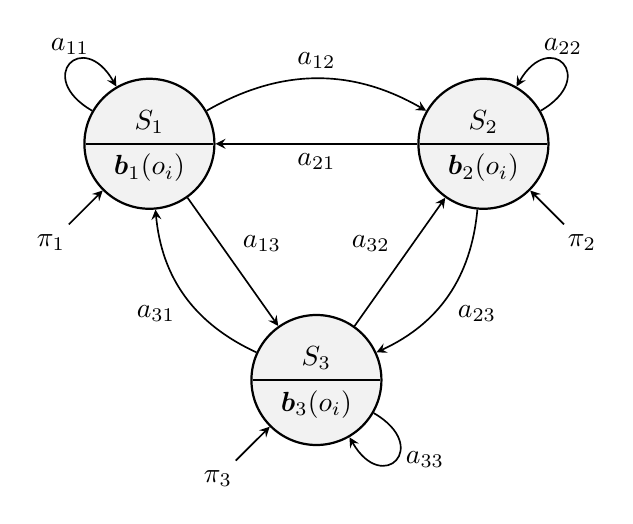
\begin{tikzpicture}[state/.style={draw, thick, circle split, fill=black!5}]
	\def\scl{1.5}
	\node[state] (S3) at (0,0) {$S_3$\nodepart{lower}$\vec{b}_3(o_i)$};
	\node[state] (S1) at (-\scl*1.414,\scl*2) {$S_1$\nodepart{lower}$\vec{b}_1(o_i)$};
	\node[state] (S2) at (\scl*1.414,\scl*2) {$S_2$\nodepart{lower}$\vec{b}_2(o_i)$};
	\draw (S1) edge[bend left] node[] {$a_{12}$} (S2);
	\draw (S2) edge[] node[] {$a_{21}$} (S1);
	\draw (S1) edge[] node[] {$a_{13}$} (S3);
	\draw (S3) edge[bend left] node[] {$a_{31}$} (S1);
	\draw (S2) edge[bend left] node[] {$a_{23}$} (S3);
	\draw (S3) edge[] node[] {$a_{32}$} (S2);
	\draw (S1) edge [out=150,in=120,looseness=5] node[above] {$a_{11}$} (S1);
	\draw (S2) edge [out=30,in=60,looseness=5] node[above] {$a_{22}$} (S2);
	\draw (S3) edge [out=-30,in=-60,looseness=5] node[right] {$a_{33}$} (S3);
	\draw ($(S1)+(-1.25,-1.25)$) node[] {$\pi_1$} edge (S1);
	\draw ($(S2)+(1.25,-1.25)$) node[] {$\pi_2$} edge (S2);
	\draw ($(S3)+(-1.25,-1.25)$) node[] {$\pi_3$} edge (S3);
\end{tikzpicture}
\end{document}